\documentclass[12pt,a4paper]{article}
\usepackage{preamble}


\PassOptionsToPackage{
  backend=biber,
  style=numeric, % eller authoryear
  sorting=nyt,
  giveninits=true,
  maxbibnames=99,
  doi=false,isbn=false,url=true,
  dashed=false
}{biblatex}


\usepackage{preamble}
\usepackage{xcolor}
\usepackage{booktabs}
\usepackage{circuitikz}
\usepackage{float} % for [H] exact figure placement
\usetikzlibrary{arrows.meta}

\usepackage{pgfplots}
\pgfplotsset{compat=1.18}

\usepackage{amsmath}




\addbibresource{./referanser.bib}

% ------ Metadata ------
\newcommand{\institution}{FHS/Cyberingeniørskolen}
\newcommand{\laboratory}{Elektronikklaboratoriet}
\newcommand{\coursecode}{ING2508 \; Kretsteknikk}
\newcommand{\assignmentno}{H04}
\newcommand{\assignmenttype}{MÅLJOURNAL}
\newcommand{\assignmenttitle}{RL- OG RC- KRETSER}
\newcommand{\studentname}{Tor Johan Aleksandersen}
\newcommand{\partnername}{Morten Cleveland}
\newcommand{\class}{VING 78}
\newcommand{\labdate}{14. november 2025}
\newcommand{\submissiondate}{\today}

\begin{document}

% frontpage.tex
\thispagestyle{empty}
\begin{minipage}{0.15\textwidth}
    \includegraphics[height=3cm]{Media/cisk.png}
\end{minipage}%
\begin{minipage}{0.4\textwidth}
    \vspace{10ex}
    \raggedright
    {\bfseries\itshape\institution}\\
    {\bfseries\itshape\laboratory}
\end{minipage}%
\begin{minipage}{0.4\textwidth}
    \vspace{13ex}
    \raggedleft
    {\today}
\end{minipage}
\vspace{1ex}

{\noindent\rule{\textwidth}{2pt}} \\ \vspace{3ex}
\begin{center}
    {\fontsize{32}{36}\selectfont \bfseries \assignmenttype}\\[6ex]
    {\fontsize{24}{28}\selectfont \bfseries OPPGAVE \assignmentno}\\[6ex]
    {\fontsize{22}{26}\selectfont \bfseries
        \parbox{0.9\textwidth}{\centering \assignmenttitle}
    }\\[10ex]

    {\fontsize{16}{20}\selectfont \bfseries \coursecode}\\[3ex]

    {\noindent\rule{\textwidth}{2pt}} \\\vspace{5ex}

    {\fontsize{20}{24}\selectfont \bfseries AV}\\[3ex]
    {\fontsize{20}{24}\selectfont \bfseries \studentname}\\ [5ex]
\end{center}

{\noindent\rule{\textwidth}{2pt}} \\\vspace{5ex}

\begin{flushleft}
    \begin{tabular}{@{}ll}
    {\fontsize{14}{18}\selectfont \bfseries KLASSE:} & {\fontsize{14}{18}\selectfont \bfseries \class} \\
    \vspace{2ex} \\
    {\fontsize{14}{18}\selectfont \bfseries LABORATORIEGRUPPE:} & {\fontsize{14}{18}\selectfont \bfseries \studentname} \\
     & {\fontsize{14}{18}\selectfont \bfseries \partnername} \\
    \vspace{2ex} \\
    {\fontsize{14}{18}\selectfont \bfseries Forsøk utført:} & {\fontsize{14}{18}\selectfont \bfseries \labdate} \\
    {\fontsize{14}{18}\selectfont \bfseries Rapport levert:} & {\fontsize{14}{18}\selectfont \bfseries \submissiondate} \\
    \end{tabular}
\end{flushleft}
\clearpage


\pagenumbering{arabic}
\setcounter{page}{1}

\section{Instrument- og komponentliste}

\subsection{Instrumentliste}
\begin{table}[h]
    \centering
    \caption{Instrumentliste}
    \vspace{1em}
    \label{tab:instrumentliste}
    \begin{tabular}{|l|l|l|c|}
        \hline
        \rowcolor[gray]{0.9}
        \textbf{Instrument} & \textbf{Beskrivelse} & \textbf{Serie Nr.} & \textbf{Antall} \\ \hline
        Digitalt Multimeter & Fluke 8808A, 5-1/2 sifret  & 2097029 & 1 \\ \hline
        Powersupply 1 & GWINSTEK GPS-3030      & 835013 & 1 \\ \hline
        Powersupply 2 & GWINSTEK GPS-3030      & 834959 & 1 \\ \hline
    \end{tabular}
\end{table}

\subsection{Komponentliste}
\begin{table}[h]
    \centering
    \caption{Komponentliste}
    \vspace{1em}
    \label{tab:komponentliste}
    \begin{tabular}{|l|l|c|}
        \hline
        \rowcolor[gray]{0.9}
        \textbf{Komponenttype} & \textbf{Verdi} & \textbf{Antall} \\ \hline
        Motstand             & 1.5k $\Omega$        & 3 \\ \hline
        Motstand             & 3.9k $\Omega$       & 1 \\ \hline
        Motstand             & 33k $\Omega$       & 4 \\ \hline
        Potensiometer             & 100k $\Omega$       & 2 \\ \hline
        Koblingsbrett & & 1 \\ \hline
    \end{tabular}
\end{table}

\clearpage

\section{Teori}

\subsection{Kondensator}
Kondensatoren er en elektrisk komponent som kan lagre elektrisk energi i sitt dielektriske område. Komponenten har en kapasitans og spenningen over kondensatoren etter en bestemt tid bestemmes av formelen under:
\begin{equation}\label{eq:spenning_i_kondensator}
    v_C(t) = V_{F} + (V_{0} - V_{F})\cdot e^{-(t-t_0)/\tau}
\end{equation}
\noindent
$V_F$ er den endelige mulige spenningen kondensatoren kan oppnå og $V_0$ er startspenningen til kondensatoren. $\tau$ her vil være kondensatorstyrken ganget med totalresistansen sett fra kondensatoren, $\tau = R_{eq}\cdot C$. Basert på om det er en kilde i kretsen eller ikke, har vi en ladnings- og utladingsfase for kondensatoren. Vi kan generalisere formlene i tilfellene opplading og utlading. I oppladingsfasen har vi initialbetingelser som gir formel:
\[
\begin{aligned}
    V_{F} &= V_{kilde} \\
    V_{0} &= 0 \\
    t_0 &= 0 \\
    v_{C\uparrow}(t) &= V_{F} + (0 - V_{F})\cdot e^{-(t - 0)/\tau} \\
    v_{C\uparrow}(t) &= V_{F} (1 -  e^{-t/\tau})
\end{aligned}
\] 
\noindent
I utladingsfasen har vi andre initialbetingelser og vi kan utlede en formel for $v_C(t)$ i denne fasen. Her vil $t_0$ være tiden brukt i oppladingsfasen:
\[
\begin{aligned}
    V_{F} &= 0 \\
    V_{0} &= v_{C\uparrow}(t_0) \\
    t_0 &= t_0 \\
    v_{C\downarrow}(t) &= 0 + (v_{C\uparrow}(t_0) - 0)\cdot e^{-(t - t_0)/\tau} \\
    v_{C\downarrow}(t) &= v_{C\uparrow}(t_0)\cdot e^{-(t - t_0)/\tau}
\end{aligned}
\] 

\subsection{RC - krets 1}
\begin{figure}[H]\label{fig:Krets}
\centering
\begin{circuitikz}[american voltages]

    %--- Noder (svarte prikker) ---------------------------------
    % Bunn/venstre (til jord)
    \node[circle, fill=black, inner sep=1.2pt] (G)  at (0,0)  {};
    \node[circle, fill=black, inner sep=1.2pt] (T1) at (0,5)  {}; % etter batteri oppe

    % Øvre gren
    \node[circle, fill=black, inner sep=1.2pt] (A)  at (4,5)  {};
    \node[circle, fill=black, inner sep=1.2pt] (B)  at (6,5)  {};
    \node[circle, fill=black, inner sep=1.2pt] (T2) at (10,5) {};

    % Nedre gren
    \node[circle, fill=black, inner sep=1.2pt] (BR) at (10,0) {};
    \node[circle, fill=black, inner sep=1.2pt] (F)  at (5,0)  {};
    \node[circle, fill=black, inner sep=1.2pt] (E)  at (5,2)  {};

    \node[circle, fill=black, inner sep=1.2pt] (D)  at (5,4)  {};

    %--- Labels på nodene ----------------------------------------
    \node[above] at (A) {$A$};
    \node[above] at (B) {$B$};
    \node[above right] at (E) {$E$};
    \node[below] at (F) {$F$};
    \node[right] at (D) {$D$};

    %--- Jord ----------------------------------------------------
    \draw (G) node[ground] {};

    %--- Batteri B1 ----------------------------------------------
    \draw (T1) to[battery1, l_=$B_1$, a^=$10\,\text{V}$] (G);

    %--- R1 fra batteri til A ------------------------------------
    \draw (T1) to[R, l_=$R_1$, a^=$12\,\text{k}\Omega$] (A);

    %--- Åpen bryter mellom A og B -------------------------------
    % "switch" gir en mekanisk brytersymbol
    \draw (D) to[switch] (5,5);

    %--- R2 på høyre side ----------------------------------------
    \draw (B) -- (T2)
          to[R, l_=$R_2$, a^=$27\,\text{k}\Omega$] (BR);

    %--- Nedre returledning --------------------------------------
    \draw (BR) -- (F) -- (G);

    %--- Kondensator C1 mellom E og F ----------------------------
    \draw (F) to[C, l_=$C_1$, a^=$68\,\mu\text{F}$] (E);

\end{circuitikz}
\caption{Krets for beregning av opp- og utladningsfase for én eller flere kondensatorer.}
\end{figure}



Vi skal studere kretsen i to tidsintervaller hvor bryteren i node $D$ er tilkoblet node $A$ eller $B$. Når bryteren er tilkoblet node $A$ vil kondensatoren lades gjennom batteriet $B_1$. Når bryteren er tilkoblet $B$ vil kondensatoren utlade gjennom motstand $R_2$. Ladingsfasen er i tiden $0 \le t \le 10\text{s}$, og utladingsfasen i tiden $10\text{s} \le t \le 20\text{s}$. Dette skal vi gjøre i tilfellene; én kondensator, to kondensatorer i serie, og to kondensatorer i parallell.


\subsubsection{Én kondensator $C_1$}
I dette tilfellet skal $D$ til $E$ kortsluttes. Kretsen i figuren under viser den overordnede kretsen for dette tilfellet.

\begin{figure}[H]
\centering
\begin{circuitikz}[american voltages]\label{fig:en_kond_figur}

    %--- Noder (svarte prikker) ---------------------------------
    % Bunn/venstre (til jord)
    \node[circle, fill=black, inner sep=1.2pt] (G)  at (0,0)  {};
    \node[circle, fill=black, inner sep=1.2pt] (T1) at (0,5)  {}; % etter batteri oppe

    % Øvre gren
    \node[circle, fill=black, inner sep=1.2pt] (A)  at (4,5)  {};
    \node[circle, fill=black, inner sep=1.2pt] (B)  at (6,5)  {};
    \node[circle, fill=black, inner sep=1.2pt] (T2) at (10,5) {};

    % Nedre gren
    \node[circle, fill=black, inner sep=1.2pt] (BR) at (10,0) {};
    \node[circle, fill=black, inner sep=1.2pt] (F)  at (5,0)  {};
    \node[circle, fill=black, inner sep=1.2pt] (E)  at (5,2)  {};

    \node[circle, fill=black, inner sep=1.2pt] (D)  at (5,4)  {};

    %--- Labels på nodene ----------------------------------------
    \node[above] at (A) {$A$};
    \node[above] at (B) {$B$};
    \node[above right] at (E) {$E$};
    \node[below] at (F) {$F$};
    \node[right] at (D) {$D$};

    %--- Jord ----------------------------------------------------
    \draw (G) node[ground] {};

    %--- DE kortslutting

    \draw (D) to[short, -] (E);

    %--- Batteri B1 ----------------------------------------------
    \draw (T1) to[battery1, l_=$B_1$, a^=$10\,\text{V}$] (G);

    %--- R1 fra batteri til A ------------------------------------
    \draw (T1) to[R, l_=$R_1$, a^=$12\,\text{k}\Omega$] (A);

    %--- Åpen bryter mellom A og B -------------------------------
    % "switch" gir en mekanisk brytersymbol
    \draw (D) to[switch] (5,5);

    %--- R2 på høyre side ----------------------------------------
    \draw (B) -- (T2)
          to[R, l_=$R_2$, a^=$27\,\text{k}\Omega$] (BR);

    %--- Nedre returledning --------------------------------------
    \draw (BR) -- (F) -- (G);

    %--- Kondensator C1 mellom E og F ----------------------------
    \draw (F) to[C, l_=$C_1$, a^=$68\,\mu\text{F}$] (E);

\end{circuitikz}
\caption{RC krets med én kondensator}
\end{figure}


\paragraph{Ladningsprosess $0 < t \le 10\text{s}$.}
Siden vi her har en kortslutting fra node $D$ til $A$ kan vi forenkle kretsen.

\begin{figure}[H]
\centering
\begin{circuitikz}[american voltages]

    %--- Noder (svarte prikker) ---------------------------------
    % Bunn/venstre (til jord)
    \node[circle, fill=black, inner sep=1.2pt] (G)  at (0,0)  {};
    \node[circle, fill=black, inner sep=1.2pt] (T1) at (0,5)  {}; % etter batteri oppe

    % Nedre gren
    \node[circle, fill=black, inner sep=1.2pt] (F)  at (5,0)  {};

    \node[circle, fill=black, inner sep=1.2pt] (D)  at (5,5)  {};

    %--- Labels på nodene ----------------------------------------
    \node[below] at (F) {$F$};
    \node[right] at (D) {$D$};

    %--- Jord ----------------------------------------------------
    \draw (G) node[ground] {};

    %--- Batteri B1 ----------------------------------------------
    \draw (T1) to[battery1, l_=$B_1$, a^=$10\,\text{V}$] (G);

    %--- R1 fra batteri til A ------------------------------------
    \draw (T1) to[R, l_=$R_1$, a^=$12\,\text{k}\Omega$] (D);

    %--- Nedre returledning --------------------------------------
    \draw (F) -- (G);

    %--- Kondensator C1 mellom E og F ----------------------------
    \draw (F) to[C, l_=$C_1$, a^=$68\,\mu\text{F}$] (D);

\end{circuitikz}
\caption{Krets for oppladingsfase for én kondensator.}
\end{figure}

\noindent
Her lades kapasitatoren av $B_1$ gjennom $R_1$ og vi kan sette opp uttrykket for spenningen i $C_1$.
\[
\begin{aligned}
    V_C(t) &= V_F (1 -  e^ {-t/\tau}) \\
    V_F &= B_1 = 10\text{V} \\
    \tau &= R_1C \\
    \tau &= 12 \cdot 10^3 \Omega \cdot 68 \cdot 10^{-6}\text{F} \\
    \tau &= 0.816\text{s}  
\end{aligned}
\]
\noindent
Vi løser for $V_C(10)$ for å vite hvor mye spenning som kondensatoren har ved starten av utladingsfasen.
\begin{align}
    V_C(t) &= 10 \left(1 -  e^{-t/0.816}\right) \label{eq:oppgaveAFør10} \\
    V_C(10) &= 10 \left(1 -  e^{-12.25}\right) \nonumber \\
    V_C(10) &\approx 10 \nonumber
\end{align}








\paragraph{Utladingsprosess $10\text{s} \le t \le 20\text{s}$.} Her vil vi kortslutte node $D$ til $B$, kondensatoren lagrer nå en spenning og blir en spenningskilde som avtar her.

\begin{figure}[H]
\centering
\begin{circuitikz}[american voltages]

    %--- Noder (svarte prikker) ---------------------------------

    % Øvre gren
    \node[circle, fill=black, inner sep=1.2pt] (T2) at (10,5) {};

    % Nedre gren
    \node[circle, fill=black, inner sep=1.2pt] (BR) at (10,0) {};
    \node[circle, fill=black, inner sep=1.2pt] (F)  at (5,0)  {};

    \node[circle, fill=black, inner sep=1.2pt] (D)  at (5,5)  {};

    %--- Labels på nodene ----------------------------------------
    \node[below] at (F) {$F$};
    \node[left] at (D) {$D$};

    %--- Jord ----------------------------------------------------
    \draw (BR) node[ground] {};

    %--- R2 på høyre side ----------------------------------------
    \draw (D) -- (T2)
          to[R, l_=$R_2$, a^=$27\,\text{k}\Omega$] (BR);

    %--- Nedre returledning --------------------------------------
    \draw (BR) -- (F);

    %--- Kondensator C1 mellom E og F ----------------------------
    \draw (D) to[V, l_=$V$, a^=$10\text{V}$] (F);

\end{circuitikz}
\caption{Krets for utladingsfase for én kondensator.}
\end{figure}

\noindent
Her starter kondensatoren sin utlading gjennom motstand $R_2$. $V_{0}$ vil være lik $V_C(10)$ fra funksjonen i første tilfelle.
\[
\begin{aligned}
    V_C(t)&=V_{0}  e^  {-(t-10)/\tau} \\
    V_{0} &= 10V \\
    \tau &= R_2C \\
    \tau &= 27\text{k}\Omega \cdot 68 \cdot 10^{-6} \\
    \tau &= 1.836
\end{aligned}
\]
\begin{equation}
    \label{eq:oppgaveAEtter10}
    V_C(t)=10 e^ {-(t-10)/1.836}
\end{equation}

\paragraph{Endelig løsning. }
Nå har vi to uttrykk for før og etter bryterskiftet. Denne funksjonen beskriver spenning over $DF$ på kretsen i figur~\ref{fig:en_kond_figur} i tidsintervallet $0 \le t \le 20\text{s}$. Dette er da ligning~\ref{eq:oppgaveAFør10} og ligning~\ref{eq:oppgaveAEtter10} med sine respektive tider:
\begin{equation}
V_C(t) =
\begin{cases}
10 \left(1 -  e^{-t/0.816}\right), & 0 \le t \le 10\text{s}, \\
10 e^{-(t-10)/1.836} & 10\text{s} < t \le 20\text{s}.
\end{cases}
\end{equation}


\subsubsection{To kondensatorer i seriekobling}\label{subsec:tilfelle2iSerie}
Kretsen figur~\ref{fig:Krets} har en ny kondensator $C_2$ mellom node $E$ og $D$. Den har samme verdi som $C_1$. Kretsen blir seende slik ut nå:

\begin{figure}[H]
\centering
\begin{circuitikz}[american voltages]

    %--- Noder (svarte prikker) ---------------------------------
    % Bunn/venstre (til jord)
    \node[circle, fill=black, inner sep=1.2pt] (G)  at (0,0)  {};
    \node[circle, fill=black, inner sep=1.2pt] (T1) at (0,5)  {}; % etter batteri oppe

    % Øvre gren
    \node[circle, fill=black, inner sep=1.2pt] (A)  at (4,5)  {};
    \node[circle, fill=black, inner sep=1.2pt] (B)  at (6,5)  {};
    \node[circle, fill=black, inner sep=1.2pt] (T2) at (10,5) {};

    % Nedre gren
    \node[circle, fill=black, inner sep=1.2pt] (BR) at (10,0) {};
    \node[circle, fill=black, inner sep=1.2pt] (F)  at (5,0)  {};
    \node[circle, fill=black, inner sep=1.2pt] (E)  at (5,2)  {};

    \node[circle, fill=black, inner sep=1.2pt] (D)  at (5,4)  {};

    %--- Labels på nodene ----------------------------------------
    \node[above] at (A) {$A$};
    \node[above] at (B) {$B$};
    \node[above right] at (E) {$E$};
    \node[below] at (F) {$F$};
    \node[right] at (D) {$D$};

    %--- Jord ----------------------------------------------------
    \draw (G) node[ground] {};

    %--- Batteri B1 ----------------------------------------------
    \draw (T1) to[battery1, l_=$B_1$, a^=$10\,\text{V}$] (G);

    %--- R1 fra batteri til A ------------------------------------
    \draw (T1) to[R, l_=$R_1$, a^=$12\,\text{k}\Omega$] (A);

    %--- Åpen bryter mellom A og B -------------------------------
    % "switch" gir en mekanisk brytersymbol
    \draw (D) to[switch] (5,5);

    %--- R2 på høyre side ----------------------------------------
    \draw (B) -- (T2)
          to[R, l_=$R_2$, a^=$27\,\text{k}\Omega$] (BR);

    %--- Nedre returledning --------------------------------------
    \draw (BR) -- (F) -- (G);

    %--- Kondensator C1 mellom E og F ----------------------------
    \draw (F) to[C, l_=$C_1$, a^=$68\,\mu\text{F}$] (E);

    %--- Kondensator C1 mellom D og E ----------------------------
    \draw (E) to[C, l_=$C_2$, a^=$68\,\mu\text{F}$] (D);

\end{circuitikz}
\caption{RC krets med to kondensatorer i seriekobling. }
\end{figure}

\noindent
I denne kretsen kan vi beskrive de ulike spenningene over $DF$. Det vil være én spenning over $C_1$, én over $C_2$ og vi kan også beskrive spenningen over hele $DF$. Siden disse er i seriekobling, strømmen vil være like over $DF$. Både $C_1$ og $C_2$ har samme strøm gjennom slik at kapasitansen i dem må være like som utledet under.
\[
\begin{aligned}
    i_{EF} &= C_1\frac{dv_{C1}}{dt} \\
    i_{DE} &= C_2\frac{dv_{C2}}{dt} \\
    i_{EF} = i_{DE} \quad &\text{og} \quad C_1 = C_2 \\
    \frac{dv_{C1}}{dt} &= \frac{dv_{C2}}{dt}
\end{aligned}
\]
\noindent
Kan vi konkludere med at spenningene må være like.
\[
v_{C1}(t) = v_{C2}(t), \qquad \text{for alle $t$}
\]
\noindent
Og vi har uttryk for alle spenningene på skinnen $DF$:
\[
\begin{aligned}
    v_{C1}(t) &= v_{C2}(t) = v_{C}(t) \\
    V_{DF}(t) &= v_{C1}(t) + v_{C2}(t) \\
    V_{DF}(t) &= 2v_{C}(t)
\end{aligned}
\]
\noindent
Nå skal vi analysere kretsen i lade- og utladingsprosessen. For å kunne bruke spenning i kondensatorformlen må vi behandle $C_1$ og $C_2$ som én totalkapasitator. Da må vi finne totalkapasitansen sett fra $DF$. $C_{tot}$ blir: $\left(C_{tot}\right)^{-1} = \left(C_1\right)^{-1} + \left(C_2\right)^{-1} \rightarrow C_{tot} = 34 \mu\text{F}$. 

\paragraph{Ladingsprosess $0 \le t \le 10\text{s}$. } Her har vi en kortslutting fra $D$ til $A$.

\begin{figure}[H]
\centering
\begin{circuitikz}[american voltages]

    %--- Noder (svarte prikker) ---------------------------------
    % Bunn/venstre (til jord)
    \node[circle, fill=black, inner sep=1.2pt] (G)  at (0,0)  {};
    \node[circle, fill=black, inner sep=1.2pt] (T1) at (0,5)  {}; % etter batteri oppe

    % Nedre gren
    \node[circle, fill=black, inner sep=1.2pt] (F)  at (5,0)  {};

    \node[circle, fill=black, inner sep=1.2pt] (D)  at (5,5)  {};

    \node[circle, fill=black, inner sep=1.2pt] (E)  at (5, 2.5)  {};

    %--- Labels på nodene ----------------------------------------
    \node[below] at (F) {$F$};
    \node[right] at (D) {$D$};
    \node[right] at (E) {$E$};

    %--- Jord ----------------------------------------------------
    \draw (G) node[ground] {};

    %--- Batteri B1 ----------------------------------------------
    \draw (T1) to[battery1, l_=$B_1$, a^=$10\,\text{V}$] (G);

    %--- R1 fra batteri til A ------------------------------------
    \draw (T1) to[R, l_=$R_1$, a^=$12\,\text{k}\Omega$] (D);

    %--- Nedre returledning --------------------------------------
    \draw (F) -- (G);

    %--- Kondensator C1 mellom E og F ----------------------------
    \draw (F) to[C, l_=$C_1$, a^=$68\,\mu\text{F}$] (E);

    %--- Kondensator C1 mellom E og D ----------------------------
    \draw (E) to[C, l_=$C_2$, a^=$68\,\mu\text{F}$] (D);

\end{circuitikz}
\caption{Krets for oppladingsfase for to kondensatorer i seriekobling. }
\end{figure}

\noindent
Vi finner \emph{tau} og uttrykket for $V_{DF}(t)$ fra sekund $0$ til $10$:
\[
\begin{aligned}
    \tau &= R_1 C_{tot} \\
    \tau &= 12\text{k}\Omega \cdot 34 \cdot 10^{-6} \\
    \tau &= 0.408\text{s} \\
    V_{DF}(t) &= V_B (1 -  e^ {-t/\tau}) \\
    V_{DF}(t) &= 10 (1 -  e^ {-t/0.408}) \\
    V_{DF}(10) &\approx 10\text{V}
\end{aligned}
\]
Her vil uttrykket for spenningen i den enkelte kondensatoren være $v_{Cn}(t) = \frac{1}{2}V_{DF}(t)$.






\paragraph{Utladingsprosess $10\text{s} \le t \le 20\text{s}$. } Her vil vi kortslutte fra $D$ til $B$ og forenkle kretsen som under.
\begin{figure}[H]
\centering
\begin{circuitikz}[american voltages]

    %--- Noder (svarte prikker) ---------------------------------

    % Øvre gren
    \node[circle, fill=black, inner sep=1.2pt] (T2) at (10,5) {};

    % Nedre gren
    \node[circle, fill=black, inner sep=1.2pt] (BR) at (10,0) {};
    \node[circle, fill=black, inner sep=1.2pt] (F)  at (5,0)  {};

    \node[circle, fill=black, inner sep=1.2pt] (D)  at (5,5)  {};
    \node[circle, fill=black, inner sep=1.2pt] (E) at (5, 2.5) {};

    %--- Labels på nodene ----------------------------------------
    \node[below] at (F) {$F$};
    \node[left] at (D) {$D$};
    \node[left] at (E) {$E$};

    %--- Jord ----------------------------------------------------
    \draw (BR) node[ground] {};

    %--- R2 på høyre side ----------------------------------------
    \draw (D) -- (T2)
          to[R, l_=$R_2$, a^=$27\,\text{k}\Omega$] (BR);

    %--- Nedre returledning --------------------------------------
    \draw (BR) -- (F);

    %--- Kondensator C1 mellom F og E ----------------------------
    \draw (E) to[V, l_=$V_1$, a^=$5\text{V}$] (F);

    %--- Kondensator C1 mellom E og D ----------------------------
    \draw (D) to[V, l_=$V_2$, a^=$5\text{V}$] (E);

\end{circuitikz}
\caption{Krets for utladingsfase for to kondensatorer i seriekobling. }
\end{figure}



\[
\begin{aligned}
    \tau &= R_2 C_{tot} \\
    \tau &= 27\text{k}\Omega \cdot 34 \cdot 10^{-6} \\
    \tau &= 0.918\text{s} \\
    V_{DF}(t) &= 10  e^ {-(t - 10)/0.918}
\end{aligned}
\]

\paragraph{Endelig uttrykk. }
\[
\begin{aligned}
    V_{DF}(t) &= 
    \begin{cases}
        10\left(1 -  e^ {-t / 0.408}\right), 0 \le t \le 10, \\ 10 e^{-(t - 10)/0.918}, 10 \le t \le 20 
    \end{cases}
    \\[1.2em]
    v_{C1}(t) = v_{C2}(t) &= 
    \begin{cases}
        5\left(1 -  e^ {-t / 0.408}\right), 0 \le t \le 10, \\ 5 e^{-(t - 10)/0.918}, 10 \le t \le 20 
    \end{cases}
\end{aligned}
\]








\subsubsection{To kondensatorer i parallellkobling}
Her skal vi kortslutte $DE$ og parallelkoble $C_2$ med $C_1$ mellom $FE$. Kretsen blir nå seende slik ut.

\begin{figure}[H]
\centering
\begin{circuitikz}[american voltages]

    %--- Noder (svarte prikker) ---------------------------------
    % Bunn/venstre (til jord)
    \node[circle, fill=black, inner sep=1.2pt] (G)  at (0,0)  {};
    \node[circle, fill=black, inner sep=1.2pt] (T1) at (0,5)  {}; % etter batteri oppe

    % Øvre gren
    \node[circle, fill=black, inner sep=1.2pt] (A)  at (4,5)  {};
    \node[circle, fill=black, inner sep=1.2pt] (B)  at (6,5)  {};
    \node[circle, fill=black, inner sep=1.2pt] (T2) at (10,5) {};

    % Nedre gren
    \node[circle, fill=black, inner sep=1.2pt] (BR) at (10,0) {};
    \node[circle, fill=black, inner sep=1.2pt] (F)  at (5,0)  {};
    \node[circle, fill=black, inner sep=1.2pt] (FL)  at (3,0)  {};
    \node[circle, fill=black, inner sep=1.2pt] (FR)  at (7,0)  {};
    \node[circle, fill=black, inner sep=1.2pt] (E)  at (5,2)  {};
    \node[circle, fill=black, inner sep=1.2pt] (EL)  at (3,2)  {};
    \node[circle, fill=black, inner sep=1.2pt] (ER)  at (7,2)  {};

    \node[circle, fill=black, inner sep=1.2pt] (D)  at (5,4)  {};

    %--- Labels på nodene ----------------------------------------
    \node[above] at (A) {$A$};
    \node[above] at (B) {$B$};
    \node[above right] at (E) {$E$};
    \node[below] at (F) {$F$};
    \node[right] at (D) {$D$};

    %--- Jord ----------------------------------------------------
    \draw (G) node[ground] {};

    %--- DE kortslutting

    \draw (D) to[short, -] (E);

    %--- Batteri B1 ----------------------------------------------
    \draw (T1) to[battery1, l_=$B_1$, a^=$10\,\text{V}$] (G);

    %--- R1 fra batteri til A ------------------------------------
    \draw (T1) to[R, l_=$R_1$, a^=$12\,\text{k}\Omega$] (A);

    %--- Åpen bryter mellom A og B -------------------------------
    % "switch" gir en mekanisk brytersymbol
    \draw (D) to[switch] (5,5);

    %--- R2 på høyre side ----------------------------------------
    \draw (B) -- (T2)
          to[R, l_=$R_2$, a^=$27\,\text{k}\Omega$] (BR);

    %--- Nedre returledning --------------------------------------
    \draw (BR) -- (F) -- (G);

    \draw (EL) -- (E) -- (ER);

    %--- Kondensator C1 mellom E og F ----------------------------
    \draw (FL) to[C, l_=$C_1$, a^=$68\,\mu\text{F}$] (EL);
    \draw (FR) to[C, l_=$C_2$, a^=$68\,\mu\text{F}$] (ER);

\end{circuitikz}
\caption{RC krets med to kondensatorer i parallellkobling. }
\end{figure}

\noindent
Her vil spenningen over $DF$ være representert av to kondensatorer i parallell. Nå kan $C_{tot}$ regnes ut som
\[
C_{tot} = C_1 + C_2 \;\;\Rightarrow\;\; C_{tot} = 136\,\mu\text{F}.
\]
Over identiske komponenter vil strømmen fordeles, men spenningen over begge kondensatorene vil være den samme siden de er parallellkoblet.
\[
v_{C1}(t) = v_{C2}(t) = V_{DF}(t).
\]

\paragraph{Ladingsprosessen $0 \le t \le 10\text{s}$. } Totalkretsen kan reduseres til kretsen under.
\begin{figure}[H]
\centering
\begin{circuitikz}[american voltages]

    %--- Noder (svarte prikker) ---------------------------------
    % Bunn/venstre (til jord)
    \node[circle, fill=black, inner sep=1.2pt] (G)  at (0,0)  {};
    \node[circle, fill=black, inner sep=1.2pt] (T1) at (0,5)  {}; % etter batteri oppe

    % Nedre gren
    \node[circle, fill=black, inner sep=1.2pt] (F)  at (5,0)  {};
    \node[circle, fill=black, inner sep=1.2pt] (FL)  at (3,0)  {};
    \node[circle, fill=black, inner sep=1.2pt] (FR)  at (7,0)  {};
    \node[circle, fill=black, inner sep=1.2pt] (E)  at (5,2)  {};
    \node[circle, fill=black, inner sep=1.2pt] (EL)  at (3,2)  {};
    \node[circle, fill=black, inner sep=1.2pt] (ER)  at (7,2)  {};

    \node[circle, fill=black, inner sep=1.2pt] (D)  at (5,5)  {};

    %--- Labels på nodene ----------------------------------------
    \node[above right] at (E) {$E$};
    \node[below] at (F) {$F$};
    \node[right] at (D) {$D$};

    %--- Jord ----------------------------------------------------
    \draw (G) node[ground] {};

    %--- DE kortslutting

    \draw (D) to[short, -] (E);

    %--- Batteri B1 ----------------------------------------------
    \draw (T1) to[battery1, l_=$B_1$, a^=$10\,\text{V}$] (G);

    %--- R1 fra batteri til A ------------------------------------
    \draw (T1) to[R, l_=$R_1$, a^=$12\,\text{k}\Omega$] (D);

    %--- Nedre returledning --------------------------------------
    \draw (G) -- (FR);

    \draw (EL) -- (E) -- (ER);

    %--- Kondensator C1 mellom E og F ----------------------------
    \draw (FL) to[C, l_=$C_1$, a^=$68\,\mu\text{F}$] (EL);
    \draw (FR) to[C, l_=$C_2$, a^=$68\,\mu\text{F}$] (ER);

\end{circuitikz}
\caption{Krets for oppladingsfasen for to kondensatorer i parallellkobling. }
\end{figure}

\noindent
Her ser vi en spenningskilde $B_1$ som lader opp en ekvivalent kapasitans $C_{tot}$ via motstanden $R_1$. Tidskonstanten og spenningen over $DF$ i ladeperioden blir
\[
\begin{aligned}
    \tau &= R_1 C_{tot} \\
    \tau &= 12\text{k}\Omega \cdot 136 \cdot 10^{-6} \\
    \tau &= 1.632\,\text{s} \\
    V_{DF}(t) &= V_B\bigl(1 -  e^{(-t/\tau)}\bigr) \\
    V_{DF}(t) &= 10\bigl(1 -  e^{(-t/1.632)}\bigr)
\end{aligned}
\]
Siden kondensatorene er parallellkoblet, har vi
\[
v_{C1}(t) = v_{C2}(t) = V_{DF}(t)
\]

\noindent
Når $t = 10\,\text{s}$ er det gått flere tidskonstanter, og vi kan ta
\[
V_{DF}(10) \approx 10\,\text{V}.
\]









\paragraph{Utladeperiode $10\text{s} \le t \le 20\text{s}$. } Kretsen blir seende slik ut:

\begin{figure}[H]
\centering
\begin{circuitikz}[american voltages]

    \node[circle, fill=black, inner sep=1.2pt] (T2) at (10,5) {};

    % Nedre gren
    \node[circle, fill=black, inner sep=1.2pt] (BR) at (10,0) {};
    \node[circle, fill=black, inner sep=1.2pt] (F)  at (5,0)  {};
    \node[circle, fill=black, inner sep=1.2pt] (FL)  at (3,0)  {};
    \node[circle, fill=black, inner sep=1.2pt] (FR)  at (7,0)  {};
    \node[circle, fill=black, inner sep=1.2pt] (E)  at (5,2)  {};
    \node[circle, fill=black, inner sep=1.2pt] (EL)  at (3,2)  {};
    \node[circle, fill=black, inner sep=1.2pt] (ER)  at (7,2)  {};

    \node[circle, fill=black, inner sep=1.2pt] (D)  at (5,5)  {};

    %--- Labels på nodene ----------------------------------------
    \node[above right] at (E) {$E$};
    \node[below] at (F) {$F$};
    \node[left] at (D) {$D$};

    %--- Jord ----------------------------------------------------
    \draw (BR) node[ground] {};

    %--- DE kortslutting

    \draw (D) to[short, -] (E);

    %--- R2 på høyre side ----------------------------------------
    \draw (D) -- (T2)
          to[R, l_=$R_2$, a^=$27\,\text{k}\Omega$] (BR);

    %--- Nedre returledning --------------------------------------
    \draw (FL) -- (BR);

    \draw (EL) -- (E) -- (ER);

    %--- Kondensator C1 mellom E og F ----------------------------
    \draw (EL) to[V, l_=$V_1$, a^=$10\text{V}$] (FL);
    \draw (ER) to[V, l_=$V_2$, a^=$10\text{V}$] (FR);

\end{circuitikz}
\caption{Krets for utladingsfasen for to kondensatorer i parallellkobling. }
\end{figure}


\noindent
Når bryteren umiddelbart etterpå kobles til node $B$, vil de to parallellkoblede kondensatorene utlades gjennom motstanden $R_2$ på samme måte som én kapasitans $C_{tot}$.
\[
\begin{aligned}
    \tau &= R_2 C_{tot} \\
    \tau &= 27\text{k}\Omega \cdot 136 \cdot 10^{-6} \\
    \tau &= 3.672\,\text{s}
    V_{DF}(t) &= V_{DF}(10)\, e^{-(t-10)/\tau} \\
    V_{DF}(t) &\approx 10\, e^{-(t-10)/3.672}
\end{aligned}
\]
Igjen er spenningen over hver av kondensatorene lik spenningen over $DF$:
\[
v_{C1}(t) = v_{C2}(t) = V_{DF}(t)
\]

\paragraph{Endelig uttrykk. }
Vi kan nå samle resultatene for hele tidsintervallet:
\[
V_{DF}(t) =
\begin{cases}
10\bigl(1 -  e^{-t/1.632}\bigr), & 0\text{s} \le t \le 10\text{s}, \\
10 e^{-(t-10)/3.672}, & 10\text{s} \le t \le 20\text{s},
\end{cases}
\]
og spenningen over hver av kondensatorene er
\[
v_{C1}(t) = v_{C2}(t) = V_{DF}(t).
\]






\subsubsection{Grafen av $V_{DF}(t)$}
Vi har tre tilfeller. Tilfelle 1-3 for kondensatorer er; én alene, to i seriekobling og to i parallellkobling. Grafing er under.

\begin{figure}[H]
\centering
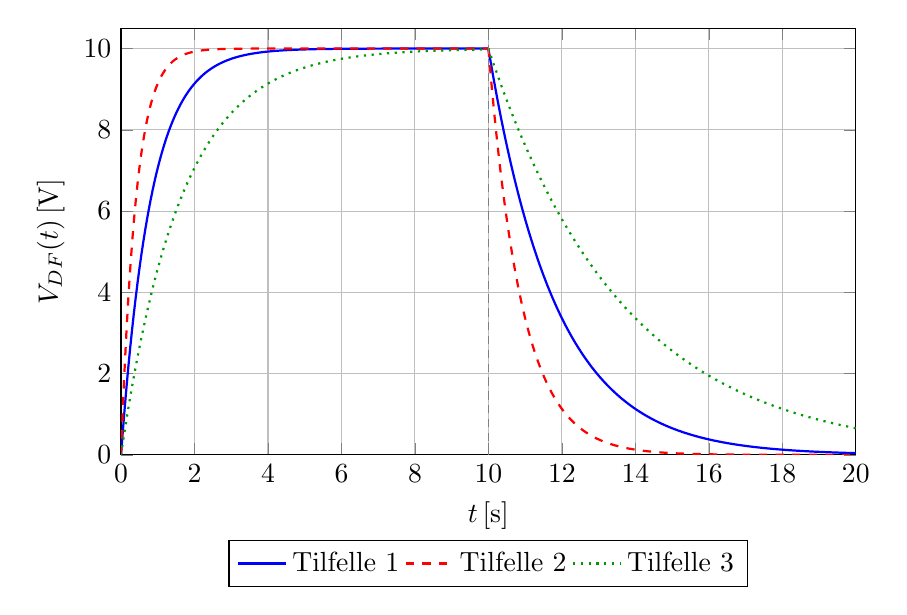
\begin{tikzpicture}
\begin{axis}[
    width=0.9\textwidth,
    height=7cm,
    xlabel={$t\,[\mathrm{s}]$},
    ylabel={$V_{DF}(t)\,[\mathrm{V}]$},
    xmin=0, xmax=20,
    ymin=0, ymax=10.5,
    grid=both,
    legend style={at={(0.5,-0.2)},anchor=north,legend columns=3},
    samples=200
]

    % --- Tilfelle 1: enkel kondensator ---
    % Lading 0–10 s
    \addplot[
        thick,
        blue,
        domain=0:10
    ]
        {10*(1 - exp(-x/0.816))};
    % Utlading 10–20 s (ikke i legend)
    \addplot[
        thick,
        blue,
        domain=10:20,
        forget plot
    ]
        {10*exp(-(x-10)/1.836)};
    \addlegendentry{Tilfelle 1}

    % --- Tilfelle 2: serie ---
    % Lading 0–10 s
    \addplot[
        thick,
        red,
        dashed,
        domain=0:10
    ]
        {10*(1 - exp(-x/0.408))};
    % Utlading 10–20 s (ikke i legend)
    \addplot[
        thick,
        red,
        dashed,
        domain=10:20,
        forget plot
    ]
        {10*exp(-(x-10)/0.918)};
    \addlegendentry{Tilfelle 2}

    % --- Tilfelle 3: parallell ---
    % Lading 0–10 s
    \addplot[
        thick,
        green!60!black,
        dotted,
        domain=0:10
    ]
        {10*(1 - exp(-x/1.632))};
    % Utlading 10–20 s (ikke i legend)
    \addplot[
        thick,
        green!60!black,
        dotted,
        domain=10:20,
        forget plot
    ]
        {10*exp(-(x-10)/3.672)};
    \addlegendentry{Tilfelle 3}

    % Vertikal linje ved t = 10 s (ikke i legend)
    \addplot[
        gray,
        densely dashed,
        forget plot
    ]
        coordinates {(10,0) (10,10.5)};

\end{axis}
\end{tikzpicture}
\caption{Spenning $V_{DF}(t)$ for tilfelle 1--3 i tidsrommet $0 \le t \le 20\,\mathrm{s}$.}
\end{figure}






\subsection{RC - krets 2}\label{subsec:rc-krets-teori}

\begin{figure}[H]\label{fig:grafet_v_av_t}
\centering
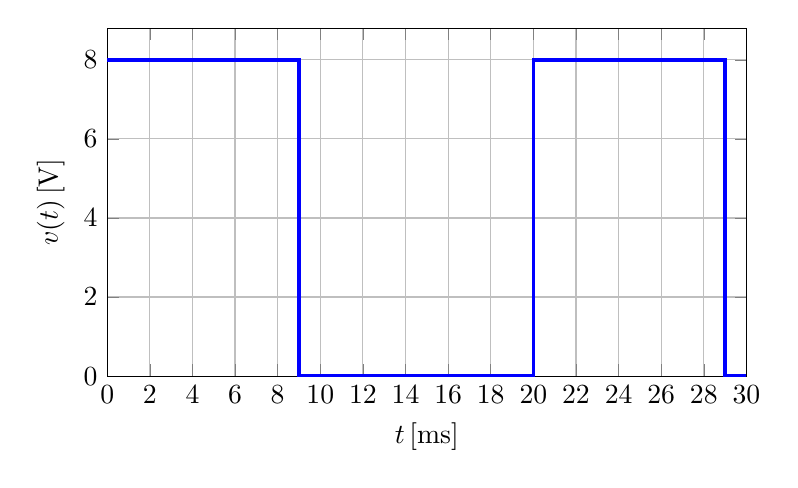
\begin{tikzpicture}
\begin{axis}[
    width=0.8\textwidth,
    height=6cm,
    xlabel={$t\,[\mathrm{ms}]$},
    ylabel={$v(t)\,[\mathrm{V}]$},
    xmin=0, xmax=30,
    ymin=0, ymax=8.8,
    ytick={0,2,4,6,8},
    xtick={0,2,...,30},
    grid=both
]
    \addplot[const plot, very thick, blue]
        coordinates {
            (0,8)
            (9,8)
            (9,0)
            (20,0)
            (20,8)
            (29,8)
            (29,0)
            (30,0)
        };
\end{axis}
\end{tikzpicture}
\caption{Inngangssignal $v(t)$ med høy-nivå $8\,\mathrm{V}$ i 9\,ms per periode.}
\end{figure}



\begin{figure}[H]\label{fig:krets-med-rc-ledd}
\centering
\begin{circuitikz}[american voltages]

    \node[circle, fill=black, inner sep=1.2pt] (BL)  at (0, 0)  {};
    \node[circle, fill=black, inner sep=1.2pt] (B)  at (5, 0)  {};
    \node[circle, fill=black, inner sep=1.2pt] (BR)  at (10, 0)  {};
    \node[circle, fill=black, inner sep=1.2pt] (TL)  at (0, 5)  {};
    \node[circle, fill=black, inner sep=1.2pt] (T)  at (5, 5)  {};
    \node[circle, fill=black, inner sep=1.2pt] (TR)  at (10, 5)  {};
    \node[circle, draw=black, fill=none, thick, inner sep=2pt] (VT)  at (12, 4)  {};
    \node[circle, draw=black, fill=none, thick, inner sep=2pt] (VB)  at (12, 1)  {};


    \node[above] at (T) {$A$};
    \node[ground] at (B) {};

    \node at (12, 3.5) {$+$};
    \node at (12, 1.5) {$-$};
    \node at (12, 2.5) {$v_0(t)$};

    \draw (TL) to[V=$v(t)$] (BL);
    \draw (TL) to[R=$2.2\text{k}\Omega$] (T);
    \draw (T) to[R=$3.9\text{k}\Omega$] (TR);
    \draw (TR) to[R, l_=$3.3\text{k}\Omega$] (BR);
    \draw (T) to[C, l_=$v_C(t)$, a^=$1\mu\text{F}$] (B);
    \draw (BL) -- (BR);

    \draw (10, 4) to[short, -] (VT);
    \draw (10, 1) to[short, -] (VB);
    


\end{circuitikz}
\caption{Kretsen i tilfelle 1}
\end{figure}



\subsubsection{DutyCycle, frekvens og symmetrilinje}
Ser vi på grafen i figur~\ref{fig:grafet_v_av_t} kan vi trekke ut DutyCycle, frekvens og symmetrilinje. Definisjonene deres er som følger:
\[
\begin{aligned}
    DutyCycle &= \frac{T_{topp}}{T_{periode}} \\
    f &= \frac{1}{T_{periode}} \\
    V_{symmetri} &= \frac{V_{min} + V_{maks}}{2}
\end{aligned}
\]
\noindent
Analyserer vi grafen ser vi at perioden er $20\text{ms}$ fordi kurven har samme tilstand, verdi og retning i enhver punkt på grafen med $20\text{ms}$ i avstand. Dette er da $T_{periode}$. Vi ser også at tiden grafen er på sin $V_{maks}$ er $9\text{ms}$. Dette er da $T_{topp}$. Grafens $V_{min}$ og $V_{maks}$ er henholdsvis $0\text{V}$ og $8\text{V}$. Da som vi har verdier løser vi for DutyCycle, frekvens og symmetrilinje under:
\[
\begin{aligned}
    T_{periode} = 20\text{ms}, \quad T_{topp} = 9\text{ms}, & \quad V_{min} = 0\text{V}, \quad V_{maks} = 8\text{V} \\[1.2em]
    DutyCycle &= \frac{9\text{ms}}{20\text{ms}} = 0.45 = 45\% \\
    f &= \frac{1}{20\text{ms}} = 50 \text{Hz} \\
    V_{sym} &= \frac{0\text{V} + 8\text{V}}{2} = 4\text{V}
\end{aligned}
\]

\subsubsection{$v_C(t)$ og $v_0(t)$ i kretsen}
$v_C(t)$ kan beskrives som spenningen ved node A. Maksimumspenning i node A kan løses for med spenningsdeling sett fra spenningskilden til node A. $R_{last}$ er totalmotstanden fra node A til jording og vi kan løse for teoretisk maksimumspenning i kondensatoren.
\[
\begin{aligned}
    R_{last} &= \left(3.9 + 3.3\right){k}\Omega \\
    R_{last} &= 7.2\text{k}\Omega
\end{aligned}
\]

\[
\begin{aligned}
    V_{A,max} &= V_{C}^{max} = 8\text{V}\cdot\frac{R_{last}}{2.2\text{k}\Omega+R_{last}} \\
    V_{A,max} &\approx 6.12\text{V}
\end{aligned}
\]

\noindent
Dette er den maksimale spenningen kondensatoren kan få hvis den får tilstrekkelig tid på å lade. Nå kan vi beregne tidskonstanten $\tau$. For dette kortslutter vi spenningskilden, dermed er det to grener til jord. $R_{eq}$ er totalmotstanden fra node A til jord.
\[
\begin{aligned}
    R_{eq} &= 2.2\text{k}\Omega || (3.9+3.3)\text{k}\Omega \\
    R_{eq} &= \frac{2.2\cdot7.2}{2.2+7.2}\text{k}\Omega \\
    R_{eq} &\approx 1.69\text{k}\Omega \\
    \tau &= R_{eq}C \approx 1.69\text{k}\Omega \cdot 1 \text{$\mu$F} \\
    \tau &\approx 1.69\text{ms}
\end{aligned}
\]

\noindent
Nå kan vi gi et uttrykk for $v_C(t)$. Først ser vi på ladefasen. Når inngangen hopper til $8\text{V}$ ved et tidspunkt $t_0$ og kondensatoren har verdi $v_C(t_0)$, får vi:
\[
v_C(t) = V_{A,max} + \left(v_C(t_0) - V_{A,max}\right) \cdot e ^{-\left(t-t_0\right)/\tau}
\]
\noindent
Men, vi har initialbetingelsen $v_C(0) = 0$ og signalet er høyt fra $t \in [0, 9\text{ms}]$. Dermed:
\[
\begin{aligned}
    v_C(t) &= V_{A,max}\left(1 -  e^{-t/\tau}\right), \qquad 0 \le t \le 9\text{ms} \\
    v_C(t) &= 6.12\left(1 -  e^{-t\cdot10^3/1.69}\right), \qquad 0 \le t \le 9\text{ms}
\end{aligned}
\]
Etter ladefasen har vi utladefasen, det vil være når $v(t)=0$. Når inngangsspenningen går til $0\text{V}$ ved $t=9\text{ms}$ vil spenningen over kondensatoren avta mot 0 med samme tidskonstant. Dette uttrykket gjelder i tidsrommet $t \in [9\text{ms}, 20\text{s}]$.
\[
\begin{aligned}
    v_C(t)&=v_C(9\text{ms}) \cdot e^ {-(t-9\text{ms})/\left(1.69\text{ms}\right)} \\
    v_C(9\text{ms})&=V_{A,max}\left(1- e^{\left(-9\text{ms}\right)/1.69\text{ms}}\right) \\
    v_C(9\text{ms})&=6.07 \\
    v_C(t) &=6.07 e^{-(t-9\text{ms})/\left(1.69\text{ms}\right)}
\end{aligned}
\]
\noindent
Nå kan vi se på et uttrykk for $v_0(t)$. Noden $v_0(t)$ ligger over motstanden $3.3\text{k}\Omega$. Dette danner en spenningsdeler sammen med $3.9\text{k}\Omega$. Vi kan bruke ligningen for spenningsdeling og regne ut $v_0(t)$.
\[
\begin{aligned}
    v_0(t)&=\frac{3.3\text{k}\Omega}{3.9\text{k}\Omega+3.3\text{k}\Omega}v_C(t) \\
    v_0(t)&\approx0.458v_C(t)
\end{aligned}
\]
\paragraph{Endelig løsning for funksjonene. } Nå som vi har uttrykt begge funksjonene i en periode. Kan vi presentere dem slik:

\[
\begin{aligned}
v_C(t) &=
\begin{cases}
6.12\bigl(1 -  e^{-{t}/{1.69\text{ms}}}\bigr), 
    & 0 \le t \le 9\text{ms},\\[0.5em]
6.07 e^{-{t - 9\text{ms}}/{1.69\text{ms}}}, 
    & 9\text{ms} \le t \le 20\text{ms},
\end{cases}
\\[1.2em]
v_0(t) &=
\begin{cases}
2.80\bigl(1 -  e^{-{t}/{1.69\text{ms}}}\bigr), 
    & 0 \le t \le 9\text{ms},\\[0.5em]
2.78 e^{-{t - 9\text{ms}}/{1.69\text{ms}}}, 
    & 9\text{ms} \le t \le 20\text{ms}.
\end{cases}
\end{aligned}
\]


\begin{figure}[H]\label{fig:teor_vC_ogv0}
\centering
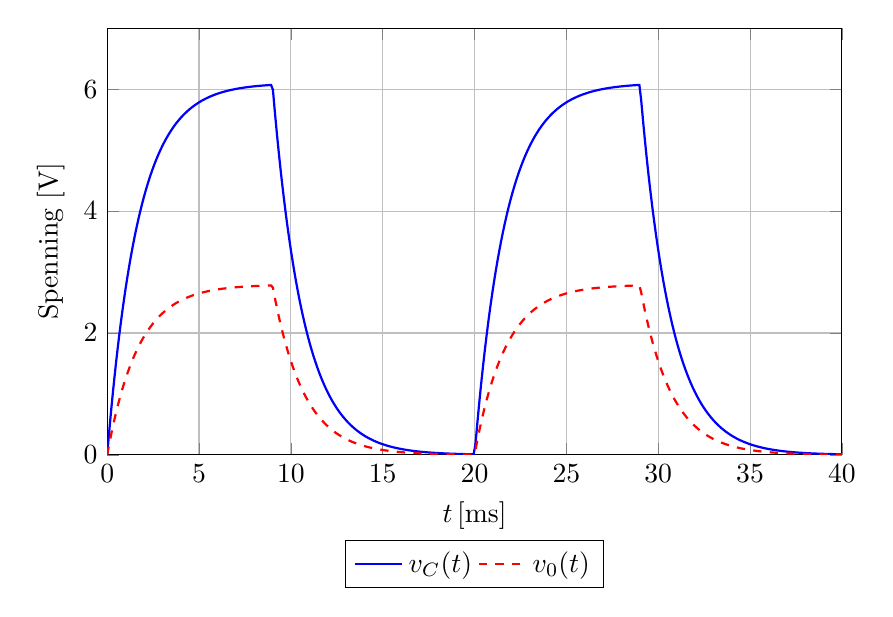
\begin{tikzpicture}
\begin{axis}[
    width=0.9\textwidth,
    height=7cm,
    xlabel={$t\,[\mathrm{ms}]$},
    ylabel={Spenning\ [V]},
    xmin=0, xmax=40,
    ymin=0, ymax=7,
    grid=both,
    legend style={at={(0.5,-0.2)},anchor=north,legend columns=2},
    samples=400
]

    % v_C(t), to perioder via mod(x,20)
    \addplot[
        thick,
        blue,
        domain=0:40
    ]
    {
        (mod(x,20) <= 9) *
            (6.1*(1 - exp(-mod(x,20)/1.69)))
        +
        (mod(x,20) > 9) *
            (6.07*exp(-(mod(x,20)-9)/1.69))
    };
    \addlegendentry{$v_C(t)$}

    % v_0(t) = 0.458 * v_C(t)
    \addplot[
        thick,
        red,
        dashed,
        domain=0:40
    ]
    {
        0.458 *
        (
            (mod(x,20) <= 9) *
                (6.1*(1 - exp(-mod(x,20)/1.69)))
            +
            (mod(x,20) > 9) *
                (6.07*exp(-(mod(x,20)-9)/1.69))
        )
    };
    \addlegendentry{$v_0(t)$}

\end{axis}
\end{tikzpicture}
\caption{Spenningene $v_C(t)$ og $v_0(t)$ over to perioder av inngangssignalet.}
\end{figure}


\subsubsection{Oppladningstida og nedladingstida for $C$}
Kondensatoren trenger mye tid for å lades helt opp eller lades helt ut, derfor er en god regel at 99.3\% av teoretisk maksverdi er regnet som fulloppladet og 0.7\% er utladet. Dette skjer etter omtrent \emph{5 tidskonstanter} begge veier.
\[
\begin{aligned}
    t &\approx 5\tau = 5 \cdot 1.69\text{ms}\\
    t &\approx 8.45\text{ms}
\end{aligned}
\]
\clearpage

\section{Gjennomføring med måleresultater}

\subsection{Måling på RC-ledd}
\subsubsection{Én kondensator}

\begin{figure}[H]
    \centering
    \includegraphics[width=0.7\textwidth]{Media/alene-C.jpeg}
    \caption{RC krets med én kondensator. Blå graf er $V_1(t)$ og gul graf er spenningen over kondensatoren.}
    \label{fig:rc_ledd_alene}
\end{figure}

\begin{figure}[H]
    \centering
    \includegraphics[width=0.7\textwidth]{Media/spenning_R4.jpeg}
    \caption{Spenningen over motstanden i RC kretsen med én kondensator.}
    \label{fig:spenning_R4}
\end{figure}









\subsubsection{To kondensatorer i serekobling}

\begin{figure}[H]
    \centering
    \includegraphics[width=0.7\textwidth]{Media/serie-C.jpeg}
    \caption{RC krets med to kondensatorer i seriekobling. Blå graf er $V_1(t)$ og gul graf er spenningen over kondensatoren.}
    \label{fig:rc_ledd_ser}
\end{figure}


\subsubsection{To kondensatorer i parallellkobling}

\begin{figure}[H]
    \centering
    \includegraphics[width=0.7\textwidth]{Media/parallell-C.jpeg}
    \caption{RC krets med to kondensatorer i parallellkobling. Blå graf er $V_1(t)$ og gul graf er spenningen over kondensatoren.}
    \label{fig:rc_ledd_par}
\end{figure}











\subsection{Måling av RL-ledd}
\begin{figure}[H]
    \centering
    \includegraphics[width=0.7\textwidth]{Media/rl-ledd-mot.jpeg}
    \caption{Resultat for måling av RL-ledd. Gul graf viser spenning over motstand og blå graf viser spenning over spolen og motstanden (totalspenningen).}
    \label{fig:rl-ledd-resultat-mot}
\end{figure}

\begin{figure}[H]
    \centering
    \includegraphics[width=0.7\textwidth]{Media/rl-ledd-spol.jpeg}
    \caption{Resultat for måling av RL-ledd. Gul graf viser spenning over spolen.}
    \label{fig:rl-ledd-resultat-spol}
\end{figure}

\subsection{Krets med RC-ledd}


\begin{figure}[H]
    \centering
    \includegraphics[width=0.7\textwidth]{Media/v_C.jpeg}
    \caption{$V_C(t)$ på oscilloskopet. $V_{\text{pp}} = 6.08\text{V}$}
    \label{fig:vc_resultat}
\end{figure}

\begin{figure}[H]
    \centering
    \includegraphics[width=0.7\textwidth]{Media/v_0.jpeg}
    \caption{$V_0(t)$ på oscilloskopet. $V_{\text{pp}} = 2.82\text{V}$}
    \label{fig:v0_resultat}
\end{figure}
\clearpage

\section{Diskusjon}

\subsection{Måling på RC-ledd}
\subsubsection{Én kondensator}
Signalgeneratoren ble stilt inn på $f=150\text{Hz}$ og amplituden målte $1.0\text{V{p-p}}$ på oscilloskopet. Kretsen under viser målingsutgangspunktet.

\begin{figure}[H]
\centering
\begin{circuitikz}[american voltages]

    \node[circle, fill=black, inner sep=1.2pt] (A)  at (0,0) {};
    \node[circle, fill=black, inner sep=1.2pt] (B)  at (0,4) {};
    \node[circle, fill=black, inner sep=1.2pt] (C)  at (8,4) {};
    \node[circle, fill=black, inner sep=1.2pt] (D)  at (8,0) {};

    \node at (A) [ground] {};
    \node at (D) [ground] {};
    \node[above left] at (B) {$A$};
    \node[above right] at (C) {$B$};
    \node[above right] at (D) {$C$};

    \draw (A) to[sV, l_=$V_1$] (B);
    \draw (B) to[R, l_=$R_4$, a^=$1\text{k}\Omega$] (C);
    \draw (C) to[C, l_=$C_7$, a^=$470\text{nF}$] (D);

\end{circuitikz}
\caption{RC krets med én kondensator.}
\end{figure}

\noindent
Resultatet i figur~\ref{fig:rc_ledd_alene} gir et godt bilde av hva som er spenningen over kondensatoren i forhold til spenningskilden. Spenningen i kondensatoren vil nærme seg firkantpulsen eksponensielt og resultatet kan vi si er godt innafor. Videre kan vi se på spenningen over motstanden $R_4$. For å kunne måle spenningen over denne motstanden må vi gjøre om på kretsen for å unngå å måle over ingen spenningsforskjell. Kretsen blir nå seende slik ut.
\begin{figure}[H]
\centering
\begin{circuitikz}[american voltages]

    \node[circle, fill=black, inner sep=1.2pt] (A)  at (0,0) {};
    \node[circle, fill=black, inner sep=1.2pt] (B)  at (0,4) {};
    \node[circle, fill=black, inner sep=1.2pt] (C)  at (8,4) {};
    \node[circle, fill=black, inner sep=1.2pt] (D)  at (8,0) {};

    \node at (A) [ground] {};
    \node at (D) [ground] {};
    \node[above left] at (B) {$A$};
    \node[above right] at (C) {$B$};
    \node[above right] at (D) {$C$};

    \draw (A) to[sV, l_=$V_1$] (B);
    \draw (C) to[R, l_=$R_4$, a^=$1\text{k}\Omega$] (D);
    \draw (B) to[C, l_=$C_7$, a^=$470\text{nF}$] (C);

\end{circuitikz}
\caption{Krets for måling av RC-ledd.}
\end{figure}

\noindent
Resultatet i figur~\ref{fig:spenning_R4} kan vi også si er riktig. Dette er fordi grafen kan forklares med å se på strømmen gjennom motstanden. Siden spenningen over motstanden beskrives som $V_R(t)$ = $R_4i(t)$. I et RC-ledd vil strømmen bestemmes av derivert spenning over kondensatoren:
\[
\begin{aligned}
    i(t)&=C\frac{dv_C(t)}{dt} \\
    v_R(t)&=RC\frac{dv_C(t)}{dt}
\end{aligned}
\]
\noindent
Nå kan vi se at spenningen over motstanden bestemmes av endringen i spenningen i kondensatoren. Derfor vil det bli stor spenning over motstanden når kondensatorspenningen stiger eller faller raskt. Når spenningen over kondensatoren flater ut vil derfor $V_R(t)$ eksponentielt synke mot null. Vi kan grafe $V_C(t)$, $V_1(t)$ og $V_R(t)$ for å se forholdet mellom dem. Ved å bruke de kjente verdiene og sette dem inn i ligning~\ref{eq:spenning_i_kondensator}.

\[
\tau = R_4 \cdot C_7 = 0.470\text{ms}
\]
\[
V_F = 1.0\text{V}
\]

\[
\begin{aligned}
v_C(t) &=
\begin{cases}
1 -  e^{-{t}/{0.470\text{ms}}}, 
    & 0 \le t \le 10\text{ms},\\[0.5em]
e^{-\left(t - 10\text{ms}\right)/{0.470\text{ms}}}, 
    & 10\text{ms} \le t \le 20\text{ms},
\end{cases}
\end{aligned}
\]

\[
v_R(t) = R_4C_7\cdot v_C'(t)
\]

\[
\begin{aligned}
v_R(t) &=
\begin{cases}
e^{-{t}/{0.470\text{ms}}}, 
    & 0 \le t \le 10\text{ms},\\[0.5em]
-e^{-\left(t - 10\text{ms}\right)/{0.470\text{ms}}}, 
    & 10\text{ms} \le t \le 20\text{ms},
\end{cases}
\end{aligned}
\]


\begin{figure}[H]
\centering
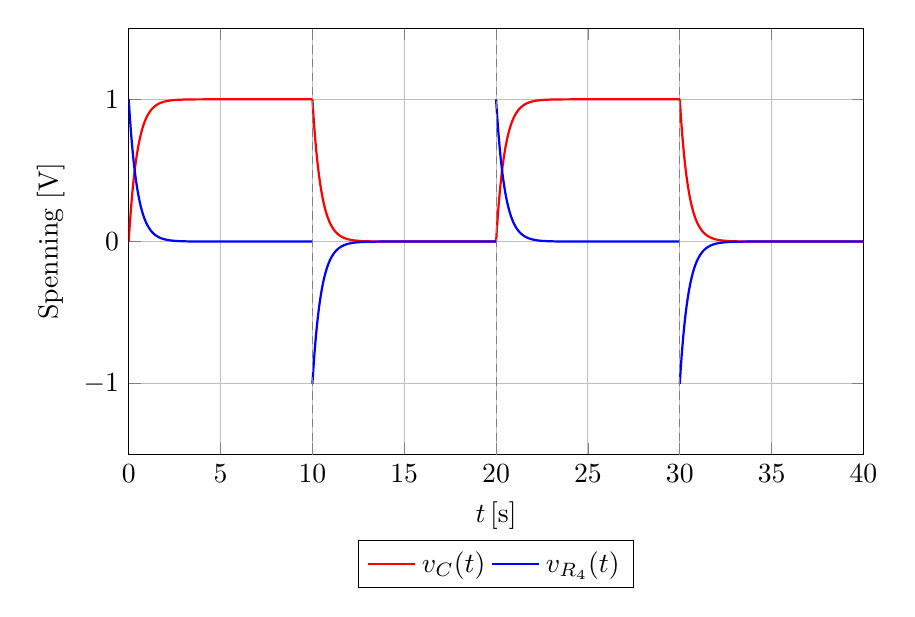
\begin{tikzpicture}
\begin{axis}[
    width=0.9\textwidth,
    height=7cm,
    xlabel={$t\,[\mathrm{s}]$},
    ylabel={Spenning\ [V]},
    xmin=0, xmax=40,
    ymin=-1.5, ymax=1.5,
    grid=both,
    legend style={at={(0.5,-0.2)},anchor=north,legend columns=2},
    samples=200
]

    % --- v_C(t): spenning over kondensatoren ---
    % Periode 1: 0–20 s
    \addplot[
        thick,
        red,
        domain=0:10
    ]
        {(1 - exp(-x/0.470))};
    \addplot[
        thick,
        red,
        domain=10:20,
        forget plot
    ]
        {exp(-(x-10)/0.470)};
    % Periode 2: 20–40 s
    \addplot[
        thick,
        red,
        domain=20:30,
        forget plot
    ]
        {(1 - exp(-(x - 20)/0.470))};
    \addplot[
        thick,
        red,
        domain=30:40,
        forget plot
    ]
        {exp(-(x-30)/0.470)};
    \addlegendentry{$v_C(t)$}

    % --- v_R4(t): spenning over motstanden R4 ---
    % Periode 1: 0–20 s
    \addplot[
        thick,
        blue,
        domain=0:10
    ]
        {exp(-x/0.470)};
    \addplot[
        thick,
        blue,
        domain=10:20,
        forget plot
    ]
        {-exp(-(x-10)/0.470)};
    % Periode 2: 20–40 s
    \addplot[
        thick,
        blue,
        domain=20:30,
        forget plot
    ]
        {exp(-(x-20)/0.470)};
    \addplot[
        thick,
        blue,
        domain=30:40,
        forget plot
    ]
        {-exp(-(x-30)/0.470)};
    \addlegendentry{$v_{R_4}(t)$}

    % Vertikale hjelpelinjer (valgfritt, ikke i legend)
    \addplot[
        gray,
        densely dashed,
        forget plot
    ]
        coordinates {(10,-1.5) (10,1.5)};
    \addplot[
        gray,
        densely dashed,
        forget plot
    ]
        coordinates {(20,-1.5) (20,1.5)};
    \addplot[
        gray,
        densely dashed,
        forget plot
    ]
        coordinates {(30,-1.5) (30,1.5)};

\end{axis}
\end{tikzpicture}
\caption{Teoretisk spenning over kondensatoren $C_T$ og motstanden $R_4$ for et firkantet inngangssignal med periode $20\,\text{s}$ og tidskonstant $\tau = 0{,}47\,\text{s}$.}
\end{figure}

\noindent
Siden dette er teoretisk tilnærming med verdiene vi har er ikke grafen helt lik den på oscilloskopet. Uansett, så bekrefter den at grafene henger sammen. Utledningen av at spenningen over motstanden er proporsjonal med endringen i spenningen på kondensatoren stemmer overens med grafen.









\subsubsection{To kondensatorer i serekobling}

\begin{figure}[H]
\centering
\begin{circuitikz}[american voltages]

    \node[circle, fill=black, inner sep=1.2pt] (A)  at (0,0) {};
    \node[circle, fill=black, inner sep=1.2pt] (B)  at (0,4) {};
    \node[circle, fill=black, inner sep=1.2pt] (C)  at (8,4) {};
    \node[circle, fill=black, inner sep=1.2pt] (D)  at (8,0) {};

    \node at (A) [ground] {};
    \node at (D) [ground] {};
    \node[above left] at (B) {$A$};
    \node[above right] at (C) {$B$};
    \node[above right] at (D) {$C$};

    \draw (A) to[sV, l_=$V_1$] (B);
    \draw (B) to[R, l_=$R_4$, a^=$1\text{k}\Omega$] (C);

    \draw (C) to[C, l_=$C_7$, a^=$470\text{nF}$] (8,2);
    \draw (8,2) to[C, l_=$C_8$, a^=$470\text{nF}$] (D);

\end{circuitikz}
\caption{RC krets med to kondensatorer i seriekobling}
\end{figure}

Resultatet på oscilloskopet i figur~\ref{fig:rc_ledd_ser} er et godt bilde av teorien. Vi må se på  totalkapasitanten for å besvare hvorfor. Totalkapasitansen i serie regnes på formen: $C_{tot}^{-1} = C_1^{-1} + \dots + C_N^{-1}$. I denne kretsen vil da totalkapasitansen være.
\[
\begin{aligned}
    C_{tot}^{-1} &= C_7^{-1} + C_8^{-1} \\
    C_{tot}^{-1} &= 2\cdot\left(470\text{nF}\right)^{-1} \\
    C_{tot} &= 235\text{nF}
\end{aligned}
\]
\noindent
Dette betyr at siden totalkapasitansen er lavere vil da tidskonstanten også være lavere, kondensatoren vil ha en lavere oppladings- og nedladingstid. Resultatet viser akkurat dette sammenliknet med bare én kondensator, siden tidskonstanten er lavere vil endringen i spenning være raskere.








\subsubsection{To kondensatorer i parallellkobling}

\begin{figure}[H]
\centering
\begin{circuitikz}[american voltages]

    \node[circle, fill=black, inner sep=1.2pt] (A)  at (0,0) {};
    \node[circle, fill=black, inner sep=1.2pt] (B)  at (0,4) {};
    \node[circle, fill=black, inner sep=1.2pt] (C)  at (8,4) {};
    \node[circle, fill=black, inner sep=1.2pt] (D)  at (4,0) {};
    \node[circle, fill=black, inner sep=1.2pt] (BL)  at (4,4) {};
    \node[circle, fill=black, inner sep=1.2pt] (DR)  at (8,0) {};

    \node at (A) [ground] {};
    \node at (D) [ground] {};
    \node[above left] at (B) {$A$};
    \node[above right] at (C) {$B$};
    \node[above right] at (D) {$C$};

    \draw (BL) -- (C);
    \draw (DR) -- (D);

    \draw (A) to[sV, l_=$V_1$] (B);
    \draw (B) to[R, l_=$R_4$, a^=$1\text{k}\Omega$] (BL);
    \draw (BL) to[C, l_=$C_7$, a^=$470\text{nF}$] (D);
    \draw (C) to[C, l_=$C_8$, a^=$470\text{nF}$] (DR);

\end{circuitikz}
\caption{RC krets med to kondensatorer i parallellkobling. }
\end{figure}

For å besvare hvorfor dette resultatet er et riktig bilde av teorien må vi se på totalkapasitanten. Totalkapasitansen her representeres av $C_1$ og $C_2$ i parallellkobling. Kondensatorer i parallellkobling vil gi en totalkapasitans av summen av dem.
\[
\begin{aligned}
    C_{tot} &= 470\text{nF} + 470\text{nF} \\
    C_{tot} &= 940\text{nF}
\end{aligned}
\]

\noindent
Denne totalkapasitanten forteller oss at tidskonstanten vil være høyere enn hva den vil være hvis det var én kondensator alene. Derfor vil kondensatorene her lades og utlades på en lavere hastighet enn ved seriekoblede kondensatorer. Derfor vil dette resultatet være et bra bilde.






\subsubsection{Sammenlikning av tilfellene}










\subsection{Måling av RL-ledd}
Kretsen for målingen av spole induktans er som i kretsen i figur~\ref{fig:rl-ledd}. Innstillingene for funksjonsgeneratoren er frekvens, $f = 100 \text{kHz}$ og amplitude slik at oscilloskopet måler $1.0V_{\text{pp}}$.
\begin{figure}[H]\label{fig:rl-ledd}
\centering
\begin{circuitikz}[american voltages]

    \node[circle, fill=black, inner sep=1.2pt] (A)  at (0,0) {};
    \node[circle, fill=black, inner sep=1.2pt] (B)  at (0,4) {};
    \node[circle, fill=black, inner sep=1.2pt] (C)  at (8,4) {};
    \node[circle, fill=black, inner sep=1.2pt] (D)  at (8,0) {};

    \node at (A) [ground] {};
    \node at (D) [ground] {};

    \node [above left] at (B) {$A$};
    \node [above right] at (C) {$B$};
    \node [right] at (D) {$C$};

    \draw (A) to[sV, l_=$V_2$, a^=$1.0 V_{pp}$] (B);

    \draw (B) to[L, l_=$L_2$, a^=$47\text{\textmu}\text{H}$] (C);

    \draw (C) to[R, l_=$R_2$, a^=$51\Omega$] (D);
    

\end{circuitikz}
\caption{Krets for måling av RL-ledd.}
\end{figure}

\noindent
Resultatene er uklare og viser ikke det ekte forholdet mellom grafene. Denne kretsen presenterer en RL-krets som består av en AC-spenningskilde, spole og motstand. I en krets som dette vil spolen motvirke endring i strøm ved å indusere en spenning. Denne spenningen vil bli synlig på oscilloskopet i totalspenningen. Ser vi på resultatene kan vi først ta for oss målingen av spenning over motstand og totalspenningen.
\\[1em]
\noindent
Resultatet er ikke riktig i form av avbilding, grafene er ikke riktig innstilt i forhold til amplitudene. Ideelt sett, dersom spenningskilden hadde vært perfekt, skulle totalspenningen i kretsen vært en ren firkantpuls, mens spenningen over motstanden skulle fulgt en eksponentiell opp- og nedgang bestemt av tidskonstanten $\tau = L / (R + R_s)$. Målingene viser derimot at totalspenningen får en tydelig topp rett etter hver overgang, og at kurven glatter seg inn mot et nivå som er lavere enn toppverdien. Samtidig ser vi at spenningen over motstanden følger den forventede eksponentielle formen, men at den ligger noe lavere enn totalspenningen i starten av pulsen.
\\[1em]
\noindent
Dette kan forklares ved at funksjonsgeneratoren i praksis ikke er en ideell spenningskilde, men har en intern motstand på omtrent $50\Omega$ og begrenset stige- og falltid. Når firkantpulsen går fra lav til høy, forsøker strømmen i kretsen å øke momentant. Spolen motvirker denne endringen ved å indusere en spenning:

\[
v_L = L\cdot \frac{di}{dt}
\]
\noindent
Denne induserte spenningen legger seg oppå kildespenningen og gjør at den målte totalspenningen får en kortvarig topp (oversving) før den avtar eksponentielt mot et stasjonært nivå. Når pulsen går fra høy til lav skjer det motsatte: spolen forsøker å opprettholde strømmen og induserer en spenning med motsatt fortegn, noe som gir et negativt “dropp” i totalspenningen.
\\[1em]
\noindent
Summen av spenningen over motstanden og spenningen over spolen er likevel lik kildespenningen til enhver tid. Det betyr at målingene er konsistente med teorien dersom vi tar hensyn til kildeimpedansen og at spenningskilden ikke er ideell. Dette forklarer hvorfor oscilloskopbildet ikke viser en perfekt firkantpuls som totalspenning, men en puls med tydelige topper ved overgangene, samtidig som formen på spenningen over motstanden stemmer godt med den teoretiske RL-responsen.
\\[1em]
\noindent
I figuren under viser vi den teoretiske spenningen over motstanden, spolen og totalspenningen i kretsen. 
Den teoretiske responsen er basert på standardligningen for en seriekoblet RL-krets
\[
L\frac{di}{dt} + (R + R_s)\,i(t) = V_s(t),
\]
der $R_s$ er funksjonsgeneratorens interne motstand. Løsningen gir en eksponentiell strømrespons med 
tidskonstant 
\[
\tau = \frac{L}{R + R_s}.
\]
Spenningene som plottes er deretter beregnet som 
\[
v_R(t) = i(t)R, \qquad 
v_L(t) = L\,\frac{di}{dt}, \qquad 
v_{\text{tot}}(t) = V_s(t) - i(t)R_s.
\]
Disse teoretiske kurvene stemmer godt overens med måleresultatene, spesielt når vi tar hensyn til 
kildeimpedansen og oscilloskopets skaleringsfeil.


\begin{figure}[H]
\centering
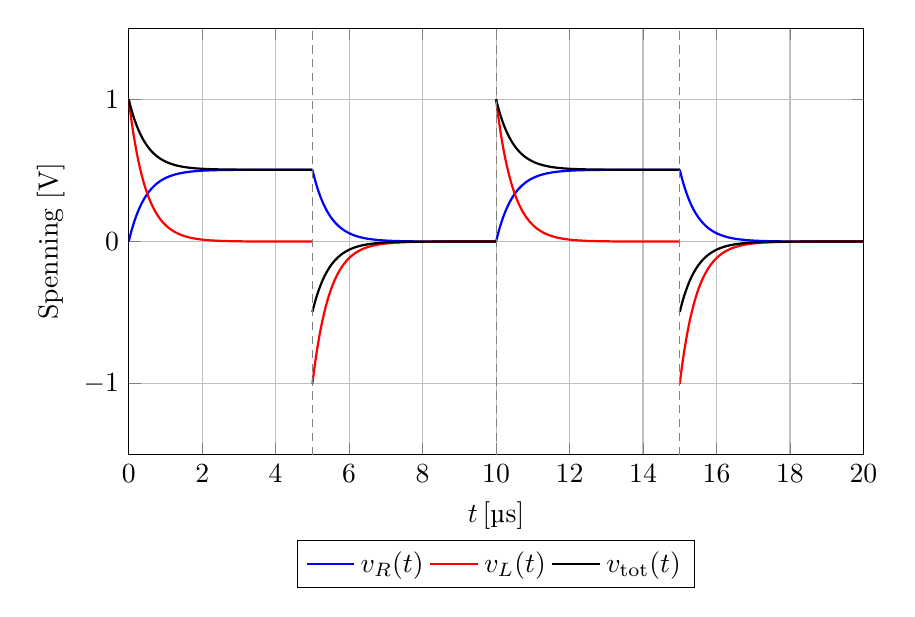
\begin{tikzpicture}
\begin{axis}[
    width=0.9\textwidth,
    height=7cm,
    xlabel={$t\,[\mathrm{\text{\textmu}s}]$},
    ylabel={Spenning\ [V]},
    xmin=0, xmax=20,
    ymin=-1.5, ymax=1.5,
    grid=both,
    legend style={at={(0.5,-0.2)},anchor=north,legend columns=3},
    samples=200
]

    % Parametre (i mikrosekund): T = 10 µs, T/2 = 5 µs, tau ≈ 0.465 µs
    % Rs = 50 Ω, R = 51 Ω
    % DC-nivåer: R/(R+Rs) ≈ 0.50495, Rs/(R+Rs) ≈ 0.49505

    % v_R(t): spenning over motstanden
    % Periode 1: 0–10 µs
    \addplot[
        thick,
        blue,
        domain=0:5
    ]
        {0.50495*(1 - exp(-x/0.465))};          % 0 <= t < 5 us
    \addplot[
        thick,
        blue,
        domain=5:10,
        forget plot
    ]
        {0.50495*exp(-(x-5)/0.465)};            % 5 <= t < 10 us
    % Periode 2: 10–20 µs
    \addplot[
        thick,
        blue,
        domain=10:15,
        forget plot
    ]
        {0.50495*(1 - exp(-(x-10)/0.465))};     % 10 <= t < 15 us
    \addplot[
        thick,
        blue,
        domain=15:20,
        forget plot
    ]
        {0.50495*exp(-(x-15)/0.465)};           % 15 <= t < 20 us
    \addlegendentry{$v_R(t)$}

    % v_L(t): spenning over spolen
    % Periode 1: 0–10 µs
    \addplot[
        thick,
        red,
        domain=0:5
    ]
        {exp(-x/0.465)};                        % 0 <= t < 5 us
    \addplot[
        thick,
        red,
        domain=5:10,
        forget plot
    ]
        {-exp(-(x-5)/0.465)};                   % 5 <= t < 10 us
    % Periode 2: 10–20 µs
    \addplot[
        thick,
        red,
        domain=10:15,
        forget plot
    ]
        {exp(-(x-10)/0.465)};                   % 10 <= t < 15 us
    \addplot[
        thick,
        red,
        domain=15:20,
        forget plot
    ]
        {-exp(-(x-15)/0.465)};                  % 15 <= t < 20 us
    \addlegendentry{$v_L(t)$}

    % v_tot(t): spenning over hele RL-leddet (det som måles som "totalspenning")
    % Periode 1: 0–10 µs
    \addplot[
        thick,
        black,
        domain=0:5
    ]
        {0.50495 + 0.49505*exp(-x/0.465)};      % 0 <= t < 5 us
    \addplot[
        thick,
        black,
        domain=5:10,
        forget plot
    ]
        {-0.49505*exp(-(x-5)/0.465)};           % 5 <= t < 10 us
    % Periode 2: 10–20 µs
    \addplot[
        thick,
        black,
        domain=10:15,
        forget plot
    ]
        {0.50495 + 0.49505*exp(-(x-10)/0.465)}; % 10 <= t < 15 us
    \addplot[
        thick,
        black,
        domain=15:20,
        forget plot
    ]
        {-0.49505*exp(-(x-15)/0.465)};          % 15 <= t < 20 us
    \addlegendentry{$v_{\text{tot}}(t)$}

    % Vertikale hjelpelinjer for T/2 og T
    \addplot[
        gray,
        densely dashed,
        forget plot
    ]
        coordinates {(5,-1.5) (5,1.5)};
    \addplot[
        gray,
        densely dashed,
        forget plot
    ]
        coordinates {(10,-1.5) (10,1.5)};
    \addplot[
        gray,
        densely dashed,
        forget plot
    ]
        coordinates {(15,-1.5) (15,1.5)};

\end{axis}
\end{tikzpicture}
\caption{Teoretisk spenning over spolen $L$, motstanden $R$ og totalspenningen $v_{\text{tot}}(t)$ i RL-kretsen med intern kilde\-motstand $R_s = 50\,\Omega$. Inngangssignalet er en firkantpuls med periode $T = 10\,\mathrm{\text{\textmu}s}$ og tidskonstant $\tau \approx 0{,}465\,\mathrm{\text{\textmu}s}$.}
\end{figure}




\subsection{Krets med RC-ledd}
Dette resultatet kommer fra teorien i~\ref{subsec:rc-krets-teori}. Resultatene presenterer målinger av akkurat denne kretsen med samme firkantpuls på spenningskilden. Resultatene må sammenliknes med figur~\ref{fig:teor_vC_ogv0}, og vi ser at resultatene stemmer. Grafen vokser og synker presist som teorien foreslår, og amplituden er riktig på både $v_c(t)$ og $v_0(t)$. Avviket er $0.16\%$ på målingen for $v_c(t)$ med en teoretisk verdi på $6.07$ og en praktisk måling på $6.08$. Avviket for $v_0(t)$ er $1.44\%$ med en praktisk måling på 2.82V og en teoretisk verdi på 2.78V. Resultatene kan vi derfor påstå at er gode og pålitelige. Grafene er riktig.
\\[1em]
Sammenhengen mellom grafene er også viktig å analysere. For å svare på hvorfor selve funksjonsoppførselen er lik, men amplituden er annerledes må vi ser på kretsen i figur~\ref{fig:krets-med-rc-ledd}. Spenningen for kondensatoren er gitt ved spenningen i node A, og spenningen over $3.3\text{k}\Omega$ motstanden er begge gitt ved to forskjellige spenningsdelere. Node A vil matematisk ha høyere spenning enn $v_0$. Dermed vil grafene oppføre seg likt i form av øking og synking, men med forskjellig hastighet og vil dermed få forskjellig amplitude i spenningen.
\clearpage

\end{document}
